%% LaTeX Beamer presentation template (requires beamer package)
%% see http://bitbucket.org/rivanvx/beamer/wiki/Home
%% idea contributed by H. Turgut Uyar
%% template based on a template by Till Tantau
%% this template is still evolving - it might differ in future releases!

\documentclass{beamer}
\usepackage[utf8]{inputenc}
\usepackage{etex}

\mode<presentation>
{
\usetheme{Boadilla}
%\usetheme{Warsaw}
\usecolortheme{wolverine}

\setbeamerfont{title}{shape=\itshape,family=\rmfamily}
\usefonttheme{serif}

\setbeamercovered{transparent}
}

\usepackage[english]{babel}

% font definitions, try \usepackage{ae} instead of the following
% three lines if you don't like this look
\usepackage{mathptmx}
\usepackage[scaled=.90]{helvet}
\usepackage{courier}
\usepackage{color}

\usepackage[T1]{fontenc}
%\usepackage{pictex}
%\usepackage{dsfont}
%\usepackage{ulem}

\title{CPCC Simulator / Gated TSP Algorithm Demo}

%\subtitle{}

% - Use the \inst{?} command only if the authors have different
%   affiliation.
%\author{F.~Author\inst{1} \and S.~Another\inst{2}}
\author{Clemens Krainer}

% - Use the \inst command only if there are several affiliations.
% - Keep it simple, no one is interested in your street address.
\institute[University of Salzburg]
{
Department of Computer Sciences\\
University of Salzburg, Austria
}

\date{June 20, 2012}


% This is only inserted into the PDF information catalog. Can be left
% out.
\subject{Talks}



% If you have a file called "university-logo-filename.xxx", where xxx
% is a graphic format that can be processed by latex or pdflatex,
% resp., then you can add a logo as follows:

% \pgfdeclareimage[height=0.5cm]{university-logo}{university-logo-filename}
% \logo{\pgfuseimage{university-logo}}



% Delete this, if you do not want the table of contents to pop up at
% the beginning of each subsection:
%\AtBeginSubsection[]
%{
%\begin{frame}<beamer>
%       \frametitle{Outline}
%       \tableofcontents[currentsection,currentsubsection]
%\end{frame}
%}

% If you wish to uncover everything in a step-wise fashion, uncomment
% the following command:

%\beamerdefaultoverlayspecification{<+->}

\begin{document}

\begin{frame}
        \titlepage
\end{frame}

\begin{frame}
        \frametitle{Outline}
        \tableofcontents
% You might wish to add the option [pausesections]
\end{frame}


\section{Demo Setup}

%\subsection[Short First Subsection Name]{First Subsection Name}

\begin{frame}\frametitle{Demo Setup} %\framesubtitle{Task}
In this demonstration four Real Vehicles (RVs) are assigned to separate square
cells. The cells are:
\vspace{0.5cm}

\begin{tabular}{|c|c|c|c|c|}
\hline
     & \multicolumn{2}{|c|}{Latitude} & \multicolumn{2}{|c|}{Longitude} \\
\hline
Cell & from    & to       & from      & to \\
\hline
 1   & 47.82202396 N & 47.82376633 N & 13.03839827 E & 13.04082245 E \\
\hline
 2   & 47.82202396 N & 47.82376633 N & 13.04082245 E & 13.04324663 E \\
\hline
 3   & 47.82028159 N & 47.82202396 N & 13.03839827 E & 13.04082245 E \\
\hline
 4   & 47.82028159 N & 47.82202396 N & 13.04082245 E & 13.04324663 E \\
\hline 
\end{tabular}

\vspace{0.5cm}
The RVs are assigned to the cells as they register with the Mapper
and each RV serves one cell exclusively and independently.  The
depot of the each RV is the center of its assigned cell.
\end{frame}

\begin{frame}\frametitle{Demo Setup}%\framesubtitle{System}
        \begin{center}
                {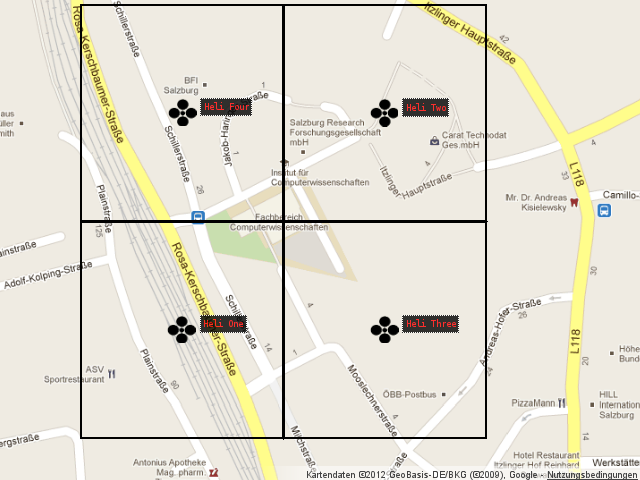
\includegraphics[width=9.5cm]{out-00000-mod.png}}
        \end{center}
\end{frame}


\section{Gated TSP Algorithm}

\begin{frame}\frametitle{Gated TSP Algorithm}\framesubtitle{RV Flight Planning }
% Each RV serves the Virtual Vehicle (VV) Action Points (APs) its own cell
% according to a gated-TSP policy as follows:
%   \begin{itemize}
%     \item With no APs to process, the RV returns to its depot and waits there
%    for new APs to appear.
% 
%     \item With APs to process, the gated-TSP mapping algorithm takes a snapshot
%   of the unprocessed APs in a RV's cell and calculates a TSP tour of those
%      APs and assigns a new flight plan to the RV.  The first waypoint of this
%      tour is the current position of the RV and the last waypoint is the RV's
%      depot position.  While RVs fly their calculated tours, the mapping
%      algorithm ignores any newly arriving APs in the according cells.
% 
%     \item After reaching the last AP of it's tour, a RV returns to its depot if
%   no more APs are to be processed (step 1) or continues to process APs (step 2).
%   \end{itemize}

For each cell the Mapper applies:

        \begin{center}
                {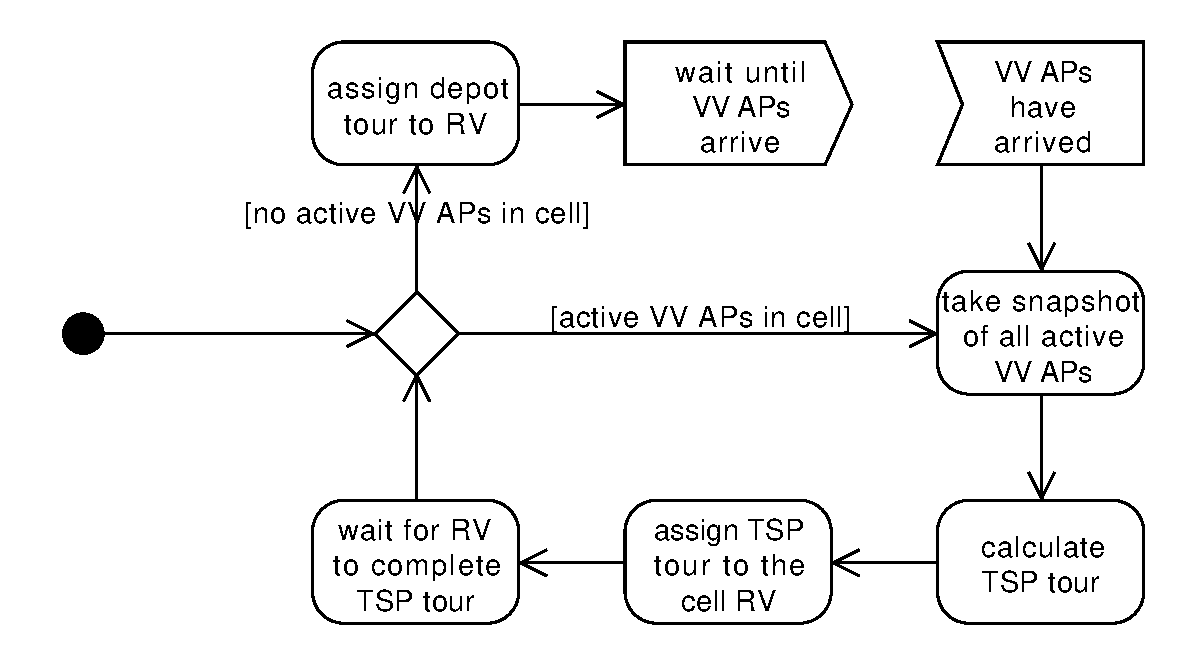
\includegraphics[width=9.5cm]{policy-2.pdf}}
        \end{center}

\end{frame}

\section{Demo}

\begin{frame}\frametitle{Demo} %\framesubtitle{Frame 000007}
% In this demonstration a small script creates 199 VVs with one randomly
% generated action point within the given cells and uploads the VVs to the
% central engine according to a Poisson process with arrival rate of one VV per 5
% seconds.

  \begin{itemize}
    \item 4 RVs in their cells. 
    \item 199 VV APs arrive randomly, average rate is one each 5 seconds.
    \item gated-TSP RV flight planning
    \item VV mapping and migration unchanged
  \end{itemize}

\end{frame}

\begin{frame}\frametitle{Demo}\framesubtitle{Frame 000007 - VV 001 arrives}
        \begin{center}
                {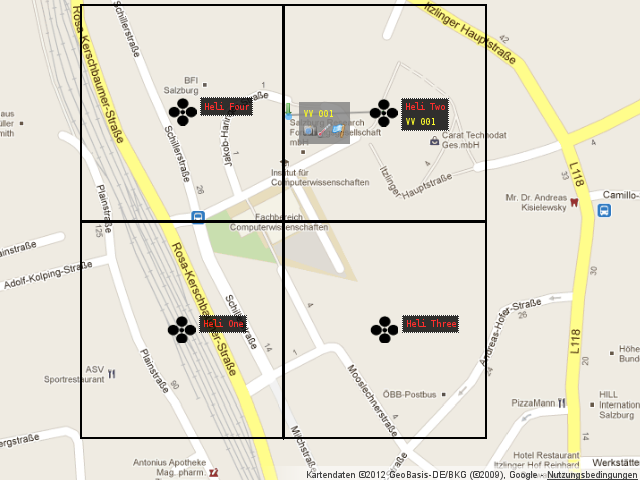
\includegraphics[width=9.5cm]{out-00007-mod.png}}
        \end{center}
\end{frame}


\begin{frame}\frametitle{Demo}\framesubtitle{Frame 000767 - TSP paths}
        \begin{center}
                {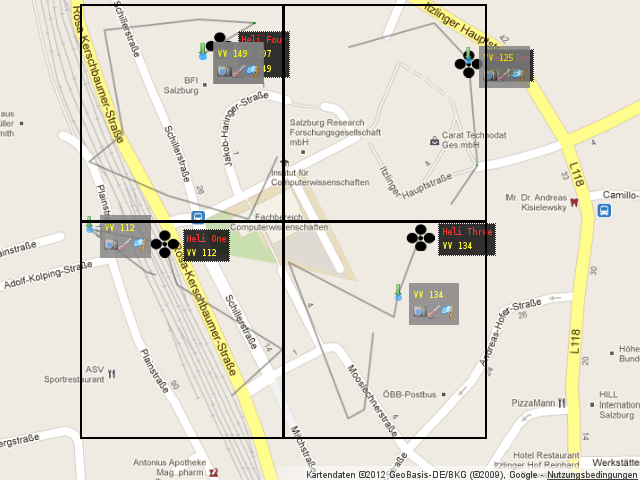
\includegraphics[width=9.5cm]{out-00767-mod.png}}
        \end{center}
\end{frame}


\begin{frame}\frametitle{Demo}\framesubtitle{Video}
%         \begin{center}
%                 {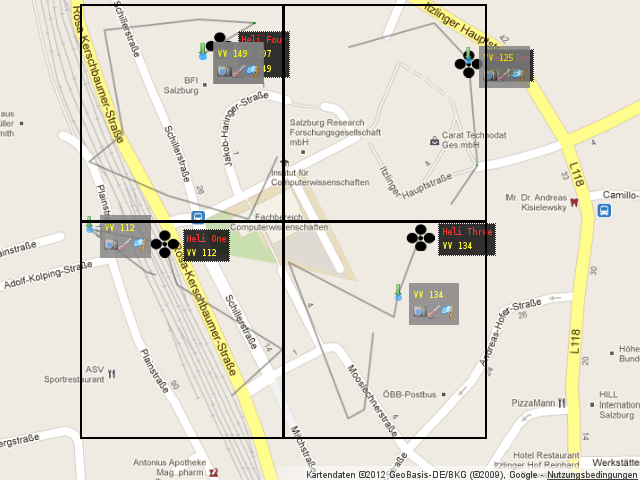
\includegraphics[width=9.5cm]{out-00767-mod.png}}
%         \end{center}
Demo Video

\end{frame}

\end{document}
